\documentclass[11pt]{article}
\usepackage{deauthor,times,graphicx}
\usepackage{url}
\def\UrlBreaks{\do\/\do-}
\usepackage{breakurl}
%\usepackage[hidelinks]{hyperref}
\usepackage{hyperref}
\usepackage{quoting}

\usepackage{xspace}

\usepackage{amsmath}
\usepackage{verbatim}
\usepackage{comment} 
\usepackage{algorithm}
\usepackage{algorithmic}
\usepackage{amsfonts}
\usepackage{amssymb}
%\usepackage{amsmath}
\usepackage{subfigure}
\usepackage{multirow}
\usepackage{flushend}
\usepackage{caption}
%\usepackage{xspace}
%\usepackage{xcolor}
%\usepackage{enumitem,url}
\usepackage{authblk}

%% BIB
%\usepackage[square, numbers]{natbib}
\usepackage{natbib}
%\setcitestyle{numbers}

\usepackage{soul,color}% highlight text with \hl{}, and to strikethrough text by \st{}
\soulregister\cite7
\soulregister\ref7
\soulregister\pageref7
\setstcolor{red}
\setul{}{.2ex}

\usepackage{graphicx}
\usepackage{xcolor}

\newcommand{\sm}[1]{\textcolor{red}{[{\bf SM: #1}]}}
\newcommand{\newsm}[1]{{\leavevmode \color{red}{#1}}}


\newcommand{\ds}[1]{\textcolor{purple}{[{\bf DS: #1}]}}
\newcommand{\newds}[1]{{\leavevmode \color{purple}{#1}}}

\definecolor{ForestGreen}{rgb}{0.13, 0.55, 0.13}
\newcommand{\newgd}[1]{{\leavevmode \color{ForestGreen}{#1}}}
\newcommand{\gd}[1]{\textcolor{ForestGreen}{[GD: #1]}}%{\relax}%put {\relax} instead to remove the 

\newcommand{\covid}{COVID-19\xspace}

\graphicspath{{authorname/}}

%%%Source of figures:
%https://app.diagrams.net/#Wb!G5-rf7UpqkWYrFzYYAHVtoKfvj-egR9OuCFnleb9C7Y--gfSuJ80RaJyCdlgoMim%2F01TP44OCXZ6WCDYRSZRZCJVCQQDI6YJJ7B

\begin{document}

\title{Human-in-the-loop Artificial Intelligence for Fighting Online Misinformation: Challenges and Opportunities}
% \title{Data Bulletin - IC7 - 10-15 pages}

\author{Gianluca Demartini$^1$, Stefano Mizzaro$^2$, Damiano Spina$^3$\\
$^1$The University of Queensland, Brisbane, Australia, g.demartini@uq.edu.au\\
$^2$University of Udine, Udine, Italy, mizzaro@uniud.it\\
$^3$RMIT University, Melbourne, Australia, damiano.spina@rmit.edu.au}

%\affil[1]{The University of Queensland, Brisbane, Australia \thanks{g.demartini@uq.edu.au}}
%\affil[2]{University of Udine, Udine, Italy \thanks{mizzaro@uniud.it}}
%\affil[3]{RMIT University, Melbourne, Australia \thanks{damiano.spina@rmit.edu.au}}

\date{}


\maketitle
\vspace{-0.2in}
\begin{abstract}
% \vspace{-0.2in}
The rise of online misinformation is posing a threat to the functioning of democratic processes. The ability to algorithmically spread false information through online social networks together with the data-driven ability to profile and micro-target individual users has made it possible to create customized false content that has the potential to influence decision making processes.
% 
Fortunately, similar data-driven and algorithmic methods can also be used to detect misinformation and to control its spread. Automatically estimating the reliability and trustworthiness of information is, however, a complex problem and it is today addressed by heavily relying on human experts known as fact-checkers.
% 
In this paper, we present the challenges and opportunities of combining automatic and manual fact-checking approaches to combat the spread on online misinformation also highlighting open research questions that the data engineering community should address.
\end{abstract}

%\newcommand{\hide}[1]{}
\section{Introduction}

As the amount of online information that is generated every day in news, social media, and the Web increases exponentially, so does the harm that false, inaccurate, or incomplete information may cause to society.
% 
Experts in fact-checking organizations are getting overwhelmed by the amount of content that requires investigation,\footnote{\url{https://www.theverge.com/2020/3/24/21192206/snopes-coronavirus-covid-19-misinformation-fact-checking-staff}} and the sophistication of bots used to generate and deliberately spread fake news and false information (i.e., disinformation) is only making the tasks carried out by experts---i.e., identifying check-worthy claims and investigating the veracity of those statements---less manageable.

The aim of this paper is to discuss the main challenges and opportunities of a hybrid approach where Artificial Intelligence (AI) tools and humans---including both experts and non-experts recruited on crowdsourcing platforms---work together to combat the spread of online misinformation.

The remainder of this paper is organized as follows. Section~\ref{sec:ai} presents an overview of human-in-the-loop AI methods. 
Section~\ref{sec:misinformation} introduces the main challenges in identifying misinformation online.
Section~\ref{sec:ML} summarizes recent work on machine learning methods applied to automatic truthfulness classification and check-worthiness.
Section~\ref{sec:crowdsourcing} describes recent advances on crowdsourcing one of the key activities in the fact-checking process, i.e., judging the truthfulness or veracity of a given statement.
Section~\ref{sec:hybrid} proposes a hybrid human-AI framework to fact-check information at scale. We conclude in
Section~\ref{sec:take-away} by summarizing the main take-away messages.





\section{Human-in-the-loop AI}
\label{sec:ai}
Human-in-the-loop AI (HAI) systems aim at leveraging the ability of AI to scale the processing to very large amounts of data while relying on human intelligence to perform very complex tasks--- for example, natural language understanding---or to incorporate fairness and/or explainability properties into the system. Example of successful HAI methods include \cite{zencrowd,crowdq,crowddb,crowdmap}. Active learning methods \cite{settles2009active} are another example of HAI where labels are collected from humans, fed back to a supervised learning model, and used to decide which data items humans should label next \cite{spina2015active}.
Related to this is the idea of interactive machine learning \cite{amershi2014power} where labels are automatically obtained from user interaction behaviors \cite{joachims2007search}.
While being more powerful than pure machine-based AI methods, HAI systems need to deal with additional challenges to perform effectively and to produce valid results. One such challenge is the possible \textit{noise} in the labels provided by humans. Depending on which human participants are providing labels for the AI component to learn from, the level of data quality may vary. For example, making use of crowdsourcing to collect human labels from people online either using paid micro-task platforms like Amazon Mechanical Turk or by means of alternative incentives like, e.g., `games with a purpose' \cite{gwap} is in general different from relying on a few experts.

There is often a trade-off between the cost and the quality of the collected labels. On the one hand, it may be possible to collect few high-quality curated labels that have been generated by domain experts, while, on the other hand, it may be possible to collect very large amounts of human-generated labels that might be not 100\% accurate. Since the number of available experts is usually limited,  to obtain both high volume and quality labels, the development of effective quality control mechanisms for crowdsourcing is needed.

Another challenge that comes with HAI systems is the \textit{bias} that contributing humans may create and/or amplify in the annotated data and, consequently, in the models learned from this labelled data \cite{hajian2016algorithmic,olteanu2019social}.
Depending on the labelling task, bias and stereotypes of contributing individuals may be reflected into the generated labels. For example, an image labelling task that requires to identify the profession of people by looking at a picture, may lead to a female individual depicted in medical attire to be labelled as `nurse' rather than as `doctor'. For such type of data collection exercises, it becomes important to measure and, if necessary, control the bias in the collected data so that the bias in the AI models trained with such data is managed and controlled as well, if not limited or avoided altogether.
Possible ways to control such bias include working on human annotator selection strategies by, for example, including pre-filtering tasks to profile annotators and to then select a balanced set of human annotators to generate labels for an AI to learn from.


Once manually labelled data has been collected, trained AI models may reflect existing bias in the data. An example of such a problem is that of `unknown unknowns' (UU) \cite{uu}, that is, data points for which a supervised model makes a high-confidence classification decision, which is however wrong. This means that the model is not aware of making mistakes. UUs are often difficult to identify because of the high-confidence of the model in its classification decision and may create critical issues in AI.\footnote{A classic example of this is the Google gorilla mistake, see \url{https://www.wired.com/story/when-it-comes-to-gorillas-google-photos-remains-blind/}.} The problem of UU is usually caused by having a part of the feature space being under-represented in the training data (e.g., training data skewed towards white male images may result into AI models that are not performing well on images of people from other ethnicities and of other genders). Thus, such AI models are biased because of the unbalanced training data they have been trained on. Possible ways to control for such bias include making use of appropriate data sampling strategies to ensure that training datasets are well balanced and cover well the feature space also for features that may not have been originally identified or used.

When incorporating humans into an HAI system, they become the efficiency bottleneck. While purely machine-based AI systems can learn from very many data points and, once trained, perform decisions in real-time, making use of a human component makes the system less scalable and less efficient. For this reason, it becomes important to decide how to best employ these less efficient and limited human resources and, instead, how to best leverage the scalability of machine-based methods in order to get the best out of the two worlds. 
% 
The problem becomes even more complex when considering different types of human contributors which come with varying quality, availability, and cost levels. We discuss this in more depth in Section \ref{sec:crowdAIexperts}.

Related to the previous problem, deciding what data points should be manually labelled by human annotators is another challenge. Given a usually very limited manual annotation budget, it becomes important to select the best data items to label in order to maximise their value with respect to the improvements of the trained AI models. Questions of this type are in particular relevant to systems relying on active learning strategies. 
Such improvements, however may relate not only to effectiveness, but also to other model properties like, for example, \textit{fairness}. 
% 
Another benefit of involving humans in HAI system is the ability to leverage their skills to improve the \textit{interpretability} and \textit{explainability} of AI models. 
Human contributors may be leveraged to, for example, add natural language explanations about \textit{why} a certain supervised classifier decision has been made. 

Thus, in order to design and develop an high-quality HAI system, researchers have to look at a multi-dimensional problem which includes aspects like efficiency, accuracy, interpretability, explainability, and fairness. Human and machine components of an HAI system can contribute and possibly threaten each of these dimensions. 
% 
Based on these issues, the overarching question in HAI systems is about deciding \textit{what should humans do} and \textit{what should AIs do} in order to optimally leverage the capabilities of both methodologies.
% 
In the remainder of this paper we discuss these challenges and opportunities in the context of fighting online misinformation. We use this problem as a showcase of HAI methods and discuss the potential of such methodology when applied to this context.


\section{The Problem of Online Misinformation}
\label{sec:misinformation}

\subsection{An Interdisciplinary Challenge}
The spread of misinformation online is a threat to our safety online and risks to damage the democratic process.
For instance, bots and trolls have been spreading disinformation across a number of significant scenarios, such as the election of US President Donald Trump in 2016 \cite{bovet2019influence}, the debate in the UK over Brexit \cite{howard2016bots}, and, more recently, exaggerating the role of arson to undermine the link between bushfires in Australia and climate change.\footnote{\url{https://theconversation.com/bushfires-bots-and-arson-claims-australia-flung-in-the-global-disinformation-spotlight-129556}} The World Health Organization (WHO) has referred to the problem of large amount of misinformation spreading during the \covid pandemic as an ``infodemic''\footnote{\url{https://www.who.int/dg/speeches/detail/director-general-s-remarks-at-the-media-briefing-on-2019-novel-coronavirus---8-february-2020}} \cite{alam2020fighting}.
Therefore, fact-checking information online is of great importance to avoid further costs to society. 

Because of the importance, impact, and interdisciplinarity of the issue, a number of different research areas have focused on understanding and stopping misinformation spreading online. This includes research in political sciences \cite{kuklinski2000misinformation}, communication science \cite{wardle2017fake}, computational social science \cite{del2016spreading}, up to computer science including the fields of human-computer interaction \cite{starbird2019disinformation}, database \cite{scrutinizer}, and information retrieval \cite{roitero2020can}. While different research methodologies are being applied, the overarching goal is to understand how misinformation is spreading, why people trust it, and how to design and test systems and processes to stop it. 

From a data engineering point of view,
online misinformation poses some of the same common challenges observed in modern data management: i)  \textit{volume}: large amounts of data to be processed efficiently and in a scalable fashion; ii) \textit{velocity}: processing data and making misinformation classification decisions in a timely fashion also in conditions when data to be checked comes as a stream (e.g., Twitter propaganda bots generating and propagating misinformation in social networks; iii) \textit{variety}: misinformation comes in multiple formats, from textual statements in news articles, to images used in social media advertising, to deep-fake videos artificially generated by AI models; iv) \textit{veracity}: the core question of truthfulness classification often translates in deciding which data source can be trusted and which not.
Thus, the data engineering community not being new to dealing with such challenges, can surely provide solutions, systems, and tools able to support the fight to online misinformation. We however still believe that this is an interdisciplinary challenge, and in the remainder of this paper we present a framework that goes beyond data engineering by including humans in the loop and by considering human factors as well.

\subsection{Misinformation Tasks}
From the existing scientific literature about misinformation, we can see that there are a number of more specific tasks that need to be addressed to achieve the overarching goal of fighting online misinformation. The first task that comes to mind is  \textit{truthfulness classification}, that is, given a statement decide its truth level, in a scale from completely true to completely false. Fully automated approaches \cite{miranda2019automated} as well as crowdsourcing-based approaches \cite{roitero2020can} have been proposed to address this task.
% 
However, other tasks  related to online misinformation exist. For example, it is also important to decide  about the \textit{check-worthiness} of online content. As there are way too many statements and claims that could possibly be fact-checked, before expert fact checking can take place, a pre-processing filtering step needs to be completed to identify which statements should be going through a complete fact-checking process, out of a large collection of potential candidates.
Criteria to be considered for such a selection process include: the potential harm that a certain statement being false could create, the reach of that statement, the importance and relevance of the topic addressed by the statement, etc.
Automated methods for check-worthiness have been proposed in the literature \cite{checkthat}, but are far from being effective enough to be deployed in practice and replace expert fact-checkers on this task.\footnote{\url{https://www.niemanlab.org/2020/07/a-lesson-in-automated-journalism-bring-back-the-humans/}}
% 
Another task related to misinformation is \textit{source identification}. Being able to detect the origin of online information can provide additional evidence to information consumers about  its level of trustworthiness.
% 
More than just either manual or automatic approaches to address these tasks, an additional way is to combine them together in order to optimize processes and leverage the best properties of each method.

\section{Machine Learning for Fighting Online Misinformation}
\label{sec:ML}
For each of the misinformation tasks described in the previous section, there have been attempts to develop machine learning methods to tackle them. In this section we provide a summary of such research.
% 
For the problem of truthfulness classification, benchmarks on which to compare the effectiveness of different approaches have been developed. A popular benchmark for truthfulness classification is the LIAR dataset \cite{wang2017liar} that makes use of expert fact-checked statements from the PolitiFact website. More than 12K expert-labeled statements are used as ground truth to train and evaluate automatic classification systems effectiveness, so that system quality can be compared.
% 
Even larger than that is the FEVER dataset \cite{thorne2018fever} that contains 180K statements obtained by altering sentences extracted from Wikipedia.
% 
Other earlier and smaller truthfulness classification benchmark datasets include \cite{vlachos2014fact,ferreira2016emergent}.

A lot of effort has been made within the AI research community not only to obtain accurate classification decision, but also to provide explainable results.
Supervised methods for this task have looked at which features are the most indicative of truthfulness \cite{reis2019supervised}. Recent approaches have designed neural networks that aim at combining evidence fragments together to inform the truthfulness classification decision \cite{wuevidence}. Such evidence  can then be used to explain the automatic classification decisions.
Other studies looking at the explainability dimension of this problem have observed that different features may be indicators for different types of fake news and can be used to cover different areas of the feature space \cite{reis2019explainable}.
Adversarial neural networks have shown to improve the effectiveness in  identifying distinctive features for truthfulness classification \cite{wu2020discovering}.

Methods to automatically decide on check-worthiness \cite{checkthat} have looked at how to assign a score to a sentence and to predict the need for it to be checked by experts using supervised methods and training data. While some methods make use of contextual information, that is, of the surrounding text, to decide on the check-worthiness of a sentence \cite{favano2019theearthisflat}, the most effective ones consider each sentence in isolation and use domain specific word embeddings within an LSTM network \cite{hansen2019neural}.

Metadata about  information sources presented to social media users have an effect on the perceived truthfulness of the information \cite{oeldorf2020posted}. Providing news source and contextual metadata may help users to make informed decisions \cite{evans2020news}. Related to this, the New York Times R\&D group has started a project to provide provenance metadata around news using blockchain technology to track the spread of news online and to provide contextual information to news readers.\footnote{\url{https://open.nytimes.com/introducing-the-news-provenance-project-723dbaf07c44}}

\section{Crowdsourcing Truthfulness}
\label{sec:crowdsourcing}
More than just machine learning-based methods, crowdsourcing can be used as a way to label data at scale. In the context of misinformation, crowdsourcing is a methodology that can provide, for example, truthfulness classification labels for statements to be fact-checked.
While experts may not be directly replaced by crowd workers (see work by \citet{bailey2008relevance}), by deploying appropriate quality control mechanisms, crowdsourcing can provide reliable labels \cite{demartini2017introduction}.
In a recent research on crowdsourcing truthfulness classification decisions we have looked at how to scale the collections of manual labels and at the impact of the annotators' background on the quality of the collected labels specifically looking for the impact of the annotator political bias with respect to the assessed statement and of the scale used to express the truthfulness judgment \cite{roitero2020can}.
% 
In another follow-up study, we have then looked at the impact of the \textit{timeliness} of the assessed statements on the quality of the collected truthfulness labels. Results show that even more recent statements can still reliably be fact-checked by the crowd \cite{roitero2020covid}. More in detail, we looked at how the crowd assessed the truthfulness of \covid true and false statements during the pandemic, finding an agreement with expert judgments comparable to that in the previous study. 
% \st{Results show that, as compared to older statements, the fact that statements are recent allows the crowd assessors to more easily identify relevant evidence that leads them to more accurate labels. }
% \sm{are we sure of this? I'd rather stay on the scale/background issues...}
% \sm{E, dopo la zoom di oggi sicuramente meglio cambiare...} \gd{ma se batch 3 e 4 sono peggio, e' un risultato consistente con quello che diciamo qui no? gli stessi statement diventano piu' vecchi e quindi meno accurati.}
% \sm{Ieri si diceva che a quanto pare sono i worker ad essere meno accurati. Se dipendesse dal tempo allora all'interno di un batch gli statement piu' sbagliati dovrebbero essere quelli vecchi, il che a quanto pare non e' (vedi figg. 22, 23)}


Another common challenge for expert fact-checkers, due to the limited available resources, is  deciding which items should be fact-checked among very many candidates.
% 
More than just leveraging crowdsourcing to decide on truthfulness, the crowd may also be able to support expert fact-checkers in performing the task of deciding about the `check-worthiness' of content, that is, asking the crowd to decide whether or not a given piece of content would benefit from being fact-checked by experts.
% 
Several factors affect the decision of selecting a statement to undergo a fact-checking process. 
The crowd may be involved in validating these factors which include,
for example, the level of public interest of the assessed content, the possible impact of such content not being true, and the timeliness of the content.
In this way, it would be possible to manually filter more content for fact-checking (the effectiveness of fully automated check-worthiness approach is still very low \cite{checkthat}) thus allowing  expert fact-checkers to focus on actual fact-checking rather than on filtering and deciding what needs to be fact-checked. 

\section{A Hybrid Human-AI Framework for Fighting Online Misinformation}
\label{sec:hybrid}

\subsection{Combining Experts, AI, and Crowd}

Given the limitations of both automated and human-based methods for fact checking, we rather envision a hybrid human-AI approach to fight online misinformation. Such an approach has the benefit of leveraging the positive aspects of each of the different approaches, that is, the scalability of AI to efficiently process very large amounts of data, the ability of expert fact-checkers to correctly identify the truthfulness level of verified statements in a transparent and fair way, and the ability of crowdsourcing to manually process significantly large datasets.
% 
We are starting to see the appearance of hybrid approaches for fact-checking, like, for example, the work presented by \citet{scrutinizer}. The proposed system is an example of how to efficiently use human fact checking resources by having a machine-based system supporting them to find the facts that need to be manually checked out of a large database of possible candidates.

The combination of these methods may not only result in more efficient and effective fact-checking processes, but also lead to improved trust on the outcomes over purely AI-based methods and may also leverage the embedded human dimension to increase the level of transparency of the truthfulness labels attached to news (i.e., explaining \textit{why} a certain piece of news has been labelled as fake, like fact-checkers do already, but something that AI-based methods still struggle to provide).
% 
Such an approach may also lead to resource optimization, where the more expensive and accurate expert fact checkers may be intelligently deployed only on the few most important and challenging verification tasks, while the crowd and AI can work together to scale-up the execution of very large amounts of fact-checking tasks.
% 
We thus envision a waterfall model where different levels of cost/quality trade-offs can be applied at different stages by means of appropriate task allocation models. 



\subsection{The Framework}
\label{sec:crowdAIexperts}

The existence of numerous challenges and constraints that need to be resolved concurrently leads us to the proposal of a solution that not only combines humans and machines, but that in doing so leverages different types and levels of engagement in the process of fighting misinformation.
% 
\begin{figure}[tb]
    \centering
    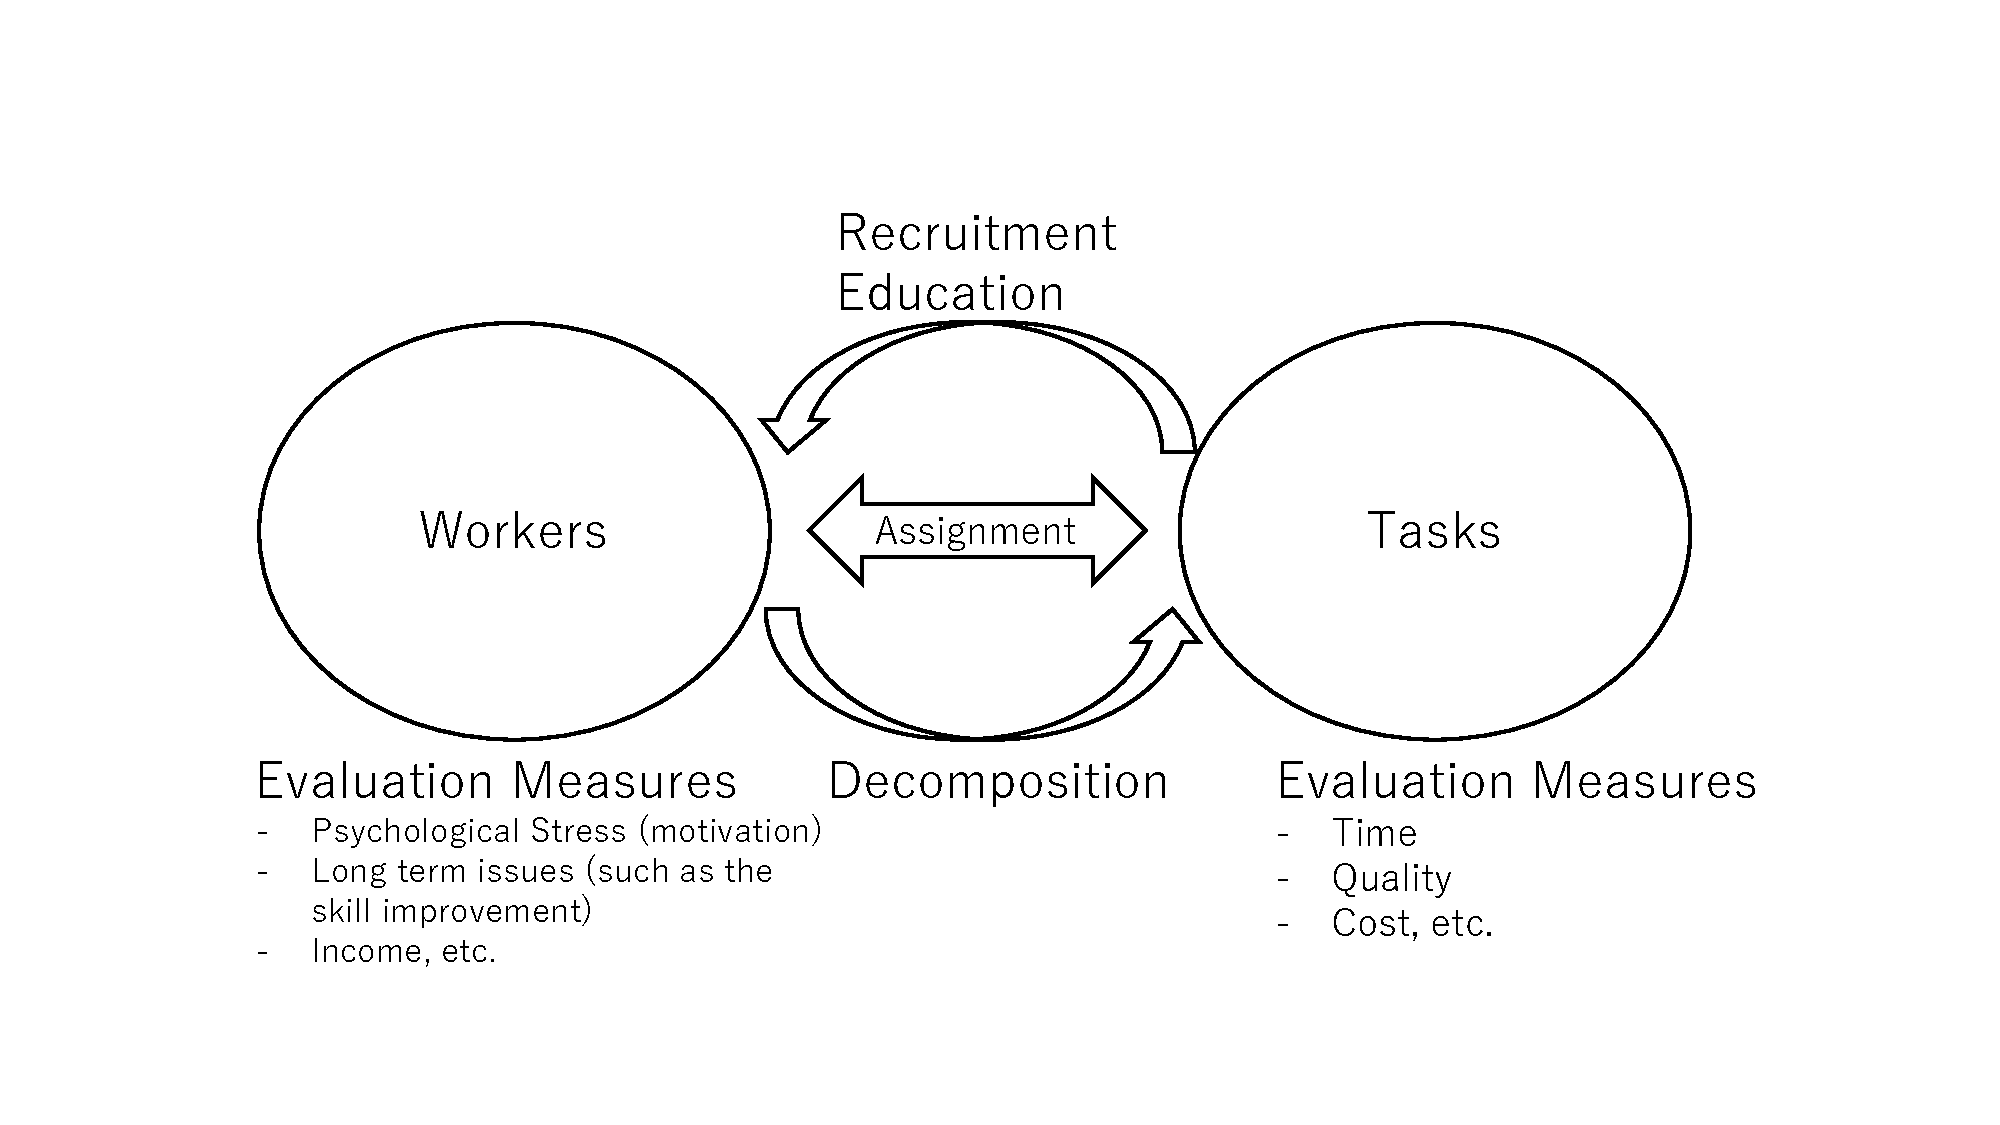
\includegraphics[width=0.7\textwidth,bb=0 0 977 506]{submissions/gianluca/figs/framework.pdf}
    \caption{Human-in-the-loop AI framework for fighting online misinformation.}
    \label{fig:framework}
\end{figure}
% 
Our proposed framework consists of three main actors: fact-checking experts, AI methods, and crowdsourcing workers (see Figure~\ref{fig:framework}). 

Fact-checking experts are the protagonists of the framework and are the ones who make use of the other two components to optimize the efficiency of the fact-checking process and maintain high-quality standards. Also, they are the only ones who can guarantee that this HAI system meets the three principles\footnote{\url{https://ifcncodeofprinciples.poynter.org/know-more/the-commitments-of-the-code-of-principles}} of (i) non-partisanship and fairness, (ii) transparency on sources, funding, and methodology; and (iii) open and honest correction policy.
% 

AI tools consist of automatic methods that fact-checkers can use to deal with the large amount of (mis)information produced through different channels such as news and media, parliamentary sessions, or social media \cite{cerone2020wnc}. Although AI tools are able to process data at  scale, automatic predictions are typically not free from errors. For instance, machine learning methods used in systems such as ClaimBuster \cite{claimbuster} or check-worthiness systems for the CheckThat! Lab at CLEF \cite{checkthat} are far from being 100\% accurate.
Moreover, it is not clear whether these tools would perform at the same level of accuracy in other scenarios, e.g., predicting check-worthiness of statements related to non-American politics.
%
In summary, although state-of-the-art machine learning can compete---and even  surpass---experts when data scale and costs are measured, as of today they are far from reaching human experts when considering the level of accuracy, explainability, and fairness.
%
\begin{figure}[tb]
    \centering
    %\includegraphics[width=0.6\textwidth,bb=0 0 546 363]{figs/framework-properties.pdf}
    \includegraphics[width=0.6\textwidth,bb=0 0 546 363]{submissions/gianluca/figs/framework-properties.pdf}
    \caption{Trade-offs between the actors of the framework.}
    \label{fig:framework-properties}
\end{figure}

Crowd workers somehow lie in between experts and AI on all the five above mentioned dimensions (scale, cost, accuracy, explainability, and control of bias) and can be deployed on-demand based on changing requirements and trade-offs. Figure~\ref{fig:framework-properties} summarizes the strong and weak points of the actors involved in the proposed framework.

The proposed framework comes with several benefits:
\begin{itemize}
    \item \textbf{Cost-quality trade-offs}: it comes with the ability to trade-off and optimize between required cost and quality of the label collection process where human experts (i.e., fact checkers) come with the highest quality and cost and AI comes with the lowest cost;
    \item \textbf{Load management}: it allows to deal with peaks of fact-checking tasks that may be otherwise impossible to deal with for expert fact-checkers working under constrained resource conditions. In such situations, they may be able to leverage the more scalable crowd and AI tools to deal with a sudden increase in annotation workload;
    \item \textbf{Trustworthiness}: it can serve as a way to make AI technology accepted in well-established traditional journalistic environments that would not see positively an `AI taking over their job'.
\end{itemize}

In such an intertwined framework, the key question becomes \textit{who should do what}. Given a workload of misinformation tasks, a deadline, and required constraints like a minimum level of quality and a maximum cost, the problem becomes to identify a task allocation solution that satisfies the constraints with maximum value.
This can be addressed with a cascade model \cite{viola2001rapid,weiss2010structured,wang2011cascade} with humans-in-the-loop, where AI tools, crowd workers and fact-checking experts cooperate to maximize value.
% 
For example, looking at the trade-off between \textit{urgency} and quality, as soon as a statement is identified as requiring fact-check, an AI model can first be adopted to very efficiently provide a truthfulness label which could then possibly be replaced later on once a team of expert fact-checkers has concluded their forensic investigation of the available evidence in favour or against the statement being true.
Such \textit{cascade of annotation tasks} where many (or all) labels are quickly estimated automatically, only a small subset of those is sent to the crowd for a quick (but non-real time) validation of their truthfulness, and then only very few remaining statements are sent to experts to investigate in depth is the core idea of the proposed framework that leverages different levels of the size-quality-cost trade-offs that the different methodologies provide.

One dimension that impacts  task allocation decisions is the cost and scale of the annotation problem. In order to leverage the best of the automated and manual methods, AI and crowdsourcing can be used to scale up the annotation effort to very many statements thus being able to possibly provide truthfulness labels for every single statement being published online. Expert fact-checkers can then be parsimoniously deployed on statements that are either difficult to label by AI or crowdsourcing methods (e.g., selected by means of low algorithmic confidence or low annotator agreement within the crowd), or important to label accurately due to the possibly wide implications of the statement being false or due to the importance of the speaker who made the statement and its potential reach.

Another open research question is on understanding how experts would actually work when embedded in this new framework: they would need to change consolidated and validated fact-checking processes and, instead,  adapt to an environment in which their work is being complemented by AI and non-experts. This would necessarily require a certain level of trust in the HAI system that, on its side, is making  decisions on what expert fact-checkers should do and on which statements they should work on. This translates into experts giving up a certain level of control on the process to the HAI system that has to decide what they do not get access to. 
For this to work, there needs to be a certain level of trust in the system that could possibly be achieved by the employment of self-explainable AI tools. This is also critical as as the fact-checking experts need at the end to be able to guarantee transparency on the process and methods used for fact-checking.




\section{Take-Away Messages}
\label{sec:take-away}

In this paper we discussed the problem of online misinformation and proposed a hybrid human-AI approach to address it.
% 
We proposed a framework that combines AI, crowdsourcing, and expert fact-checkers to produce annotations for statements by balancing annotation cost, quality, volume, and speed thus providing information consumers (e.g., social media users) with timely and accurate fact-checking results at scale.

The proposed HAI approach aims at combining different methods to leverage the best properties of both AI and human-based annotation. Moreover, involving humans in the loop allows to better deal with the interdisciplinary nature of the misinformation problem by also providing human support on issues like explainability, trust, and bias.

The  model presented in this paper envisions a complex collaborative scheme between different humans and different AIs where the open research question moves to the optimization of these complementary resources and on how to decide which task should be allocated to which element of the HAI system.
A human-in-the-loop solution to misinformation can also provide increased transparency on  fact-checking processes leveraging together algorithms and AI and, in the end, provide more evidence and power to the end users to make informed decisions on which online information they should and which they should  not  trust.


%\bibliographystyle{abbrvnat}
%\bibliography{references}
\begin{thebibliography}{10}
	\itemsep=1pt
	\begin{small}
\bibitem[Alam et~al.(2020)Alam, Shaar, Nikolov, Mubarak, Martino, Abdelali,
Dalvi, Durrani, Sajjad, Darwish, et~al.]{alam2020fighting}
F.~Alam, S.~Shaar, A.~Nikolov, H.~Mubarak, G.~D.~S. Martino, A.~Abdelali,
F.~Dalvi, N.~Durrani, H.~Sajjad, K.~Darwish, et~al.
\newblock {Fighting the COVID-19 Infodemic: Modeling the Perspective of
	Journalists, Fact-Checkers, Social Media Platforms, Policy Makers, and the
	Society}.
\newblock \emph{arXiv preprint arXiv:2005.00033}, 2020.

\bibitem[Amershi et~al.(2014)Amershi, Cakmak, Knox, and
Kulesza]{amershi2014power}
S.~Amershi, M.~Cakmak, W.~B. Knox, and T.~Kulesza.
\newblock Power to the people: The role of humans in interactive machine
learning.
\newblock \emph{AI Magazine}, 35\penalty0 (4):\penalty0 105--120, 2014.

\bibitem[Attenberg et~al.(2015)Attenberg, Ipeirotis, and Provost]{uu}
J.~Attenberg, P.~Ipeirotis, and F.~Provost.
\newblock Beat the machine: Challenging humans to find a predictive model's
“unknown unknowns”.
\newblock \emph{Journal of Data and Information Quality (JDIQ)}, 6\penalty0
(1):\penalty0 1--17, 2015.

\bibitem[Bailey et~al.(2008)Bailey, Craswell, Soboroff, Thomas, de~Vries, and
Yilmaz]{bailey2008relevance}
P.~Bailey, N.~Craswell, I.~Soboroff, P.~Thomas, A.~P. de~Vries, and E.~Yilmaz.
\newblock Relevance assessment: Are judges exchangeable and does it matter?
\newblock In \emph{Proceedings of SIGIR}, pages 667--674, 2008.

\bibitem[Bovet and Makse(2019)]{bovet2019influence}
A.~Bovet and H.~A. Makse.
\newblock {Influence of fake news in Twitter during the 2016 US presidential
	election}.
\newblock \emph{Nature communications}, 10\penalty0 (1):\penalty0 1--14, 2019.

\bibitem[Cerone et~al.(2020)Cerone, Naghizade, Scholer, Mallal, Skelton, and
Spina]{cerone2020wnc}
A.~Cerone, E.~Naghizade, F.~Scholer, D.~Mallal, R.~Skelton, and D.~Spina.
\newblock {Watch 'n' Check}: Towards a social media monitoring tool to assist
fact-checking experts.
\newblock In \emph{Proceedings of DSAA}, 2020.

\bibitem[Del~Vicario et~al.(2016)Del~Vicario, Bessi, Zollo, Petroni, Scala,
Caldarelli, Stanley, and Quattrociocchi]{del2016spreading}
M.~Del~Vicario, A.~Bessi, F.~Zollo, F.~Petroni, A.~Scala, G.~Caldarelli, H.~E.
Stanley, and W.~Quattrociocchi.
\newblock The spreading of misinformation online.
\newblock \emph{PNAS}, 113\penalty0 (3):\penalty0 554--559, 2016.

\bibitem[Demartini et~al.(2012)Demartini, Difallah, and
Cudr{\'e}-Mauroux]{zencrowd}
G.~Demartini, D.~E. Difallah, and P.~Cudr{\'e}-Mauroux.
\newblock Zencrowd: leveraging probabilistic reasoning and crowdsourcing
techniques for large-scale entity linking.
\newblock In \emph{Proceedings of the 21st international conference on World
	Wide Web}, pages 469--478, 2012.

\bibitem[Demartini et~al.(2013)Demartini, Trushkowsky, Kraska, Franklin, and
Berkeley]{crowdq}
G.~Demartini, B.~Trushkowsky, T.~Kraska, M.~J. Franklin, and U.~Berkeley.
\newblock Crowdq: Crowdsourced query understanding.
\newblock In \emph{CIDR}, 2013.

\bibitem[Demartini et~al.(2017)Demartini, Difallah, Gadiraju, and
Catasta]{demartini2017introduction}
G.~Demartini, D.~E. Difallah, U.~Gadiraju, and M.~Catasta.
\newblock An introduction to hybrid human-machine information systems.
\newblock \emph{Foundations and Trends in Web Science}, 7\penalty0
(1):\penalty0 1--87, 2017.

\bibitem[Elsayed et~al.(2019)Elsayed, Nakov, Barr{\'o}n-Cedeno, Hasanain,
Suwaileh, Da~San~Martino, and Atanasova]{checkthat}
T.~Elsayed, P.~Nakov, A.~Barr{\'o}n-Cedeno, M.~Hasanain, R.~Suwaileh,
G.~Da~San~Martino, and P.~Atanasova.
\newblock Overview of the {CLEF-2019 CheckThat! Lab}: Automatic identification
and verification of claims.
\newblock In \emph{Proceedings of CLEF}, pages 301--321, 2019.

\bibitem[Evans et~al.(2020)Evans, Edge, Larson, and White]{evans2020news}
N.~Evans, D.~Edge, J.~Larson, and C.~White.
\newblock News provenance: Revealing news text reuse at web-scale in an
augmented news search experience.
\newblock In \emph{Proceedings of CHI}, pages 1--8, 2020.

\bibitem[Favano et~al.(2019)Favano, Carman, and
Lanzi]{favano2019theearthisflat}
L.~Favano, M.~J. Carman, and P.~L. Lanzi.
\newblock {TheEarthIsFlat's submission to CLEF'19 CheckThat! challenge}.
\newblock In \emph{CLEF (Working Notes)}, 2019.

\bibitem[Ferreira and Vlachos(2016)]{ferreira2016emergent}
W.~Ferreira and A.~Vlachos.
\newblock Emergent: a novel data-set for stance classification.
\newblock In \emph{Proceedings of NAACL-HLT}, pages 1163--1168, 2016.

\bibitem[Franklin et~al.(2011)Franklin, Kossmann, Kraska, Ramesh, and
Xin]{crowddb}
M.~J. Franklin, D.~Kossmann, T.~Kraska, S.~Ramesh, and R.~Xin.
\newblock Crowddb: answering queries with crowdsourcing.
\newblock In \emph{Proceedings of the 2011 ACM SIGMOD International Conference
	on Management of data}, pages 61--72, 2011.

\bibitem[Hajian et~al.(2016)Hajian, Bonchi, and
Castillo]{hajian2016algorithmic}
S.~Hajian, F.~Bonchi, and C.~Castillo.
\newblock Algorithmic bias: From discrimination discovery to fairness-aware
data mining.
\newblock In \emph{Proceedings of KDD}, pages 2125--2126, 2016.

\bibitem[Hansen et~al.(2019)Hansen, Hansen, Alstrup, Grue~Simonsen, and
Lioma]{hansen2019neural}
C.~Hansen, C.~Hansen, S.~Alstrup, J.~Grue~Simonsen, and C.~Lioma.
\newblock Neural check-worthiness ranking with weak supervision: Finding
sentences for fact-checking.
\newblock In \emph{Proceedings of TheWebConf}, pages 994--1000, 2019.

\bibitem[Hassan et~al.(2017)Hassan, Zhang, Arslan, Caraballo, Jimenez, Gawsane,
Hasan, Joseph, Kulkarni, Nayak, et~al.]{claimbuster}
N.~Hassan, G.~Zhang, F.~Arslan, J.~Caraballo, D.~Jimenez, S.~Gawsane, S.~Hasan,
M.~Joseph, A.~Kulkarni, A.~K. Nayak, et~al.
\newblock {ClaimBuster}: The first-ever end-to-end fact-checking system.
\newblock \emph{Proceedings of the VLDB Endowment}, 10\penalty0 (12):\penalty0
1945--1948, 2017.

\bibitem[Howard and Kollanyi(2016)]{howard2016bots}
P.~N. Howard and B.~Kollanyi.
\newblock {Bots, \#StrongerIn, and \#Brexit: Computational propaganda during
	the UK-EU referendum}.
\newblock \emph{Available at SSRN 2798311}, 2016.

\bibitem[Joachims and Radlinski(2007)]{joachims2007search}
T.~Joachims and F.~Radlinski.
\newblock Search engines that learn from implicit feedback.
\newblock \emph{Computer}, 40\penalty0 (8):\penalty0 34--40, 2007.

\bibitem[Karagiannis et~al.(2020)Karagiannis, Saeed, Papotti, and
Trummer]{scrutinizer}
G.~Karagiannis, M.~Saeed, P.~Papotti, and I.~Trummer.
\newblock Scrutinizer: A mixed-initiative approach to large-scale, data-driven
claim verification.
\newblock \emph{Proceedings of the VLDB Endowment}, 13\penalty0 (11):\penalty0
2508--2521, 2020.

\bibitem[Kuklinski et~al.(2000)Kuklinski, Quirk, Jerit, Schwieder, and
Rich]{kuklinski2000misinformation}
J.~H. Kuklinski, P.~J. Quirk, J.~Jerit, D.~Schwieder, and R.~F. Rich.
\newblock Misinformation and the currency of democratic citizenship.
\newblock \emph{Journal of Politics}, 62\penalty0 (3):\penalty0 790--816, 2000.

\bibitem[Miranda et~al.(2019)Miranda, Nogueira, Mendes, Vlachos, Secker,
Garrett, Mitchel, and Marinho]{miranda2019automated}
S.~Miranda, D.~Nogueira, A.~Mendes, A.~Vlachos, A.~Secker, R.~Garrett,
J.~Mitchel, and Z.~Marinho.
\newblock Automated fact checking in the news room.
\newblock In \emph{Proceedings of TheWebConf}, pages 3579--3583, 2019.

\bibitem[Oeldorf-Hirsch and DeVoss(2020)]{oeldorf2020posted}
A.~Oeldorf-Hirsch and C.~L. DeVoss.
\newblock Who posted that story? processing layered sources in facebook news
posts.
\newblock \emph{Journalism \& Mass Communication Quarterly}, 97\penalty0
(1):\penalty0 141--160, 2020.

\bibitem[Olteanu et~al.(2019)Olteanu, Castillo, Diaz, and
Kiciman]{olteanu2019social}
A.~Olteanu, C.~Castillo, F.~Diaz, and E.~Kiciman.
\newblock Social data: Biases, methodological pitfalls, and ethical boundaries.
\newblock \emph{Frontiers in Big Data}, 2:\penalty0 13, 2019.

\bibitem[Reis et~al.(2019{\natexlab{a}})Reis, Correia, Murai, Veloso, and
Benevenuto]{reis2019explainable}
J.~C. Reis, A.~Correia, F.~Murai, A.~Veloso, and F.~Benevenuto.
\newblock Explainable machine learning for fake news detection.
\newblock In \emph{Proceedings of WebSci}, pages 17--26, 2019{\natexlab{a}}.

\bibitem[Reis et~al.(2019{\natexlab{b}})Reis, Correia, Murai, Veloso, and
Benevenuto]{reis2019supervised}
J.~C. Reis, A.~Correia, F.~Murai, A.~Veloso, and F.~Benevenuto.
\newblock Supervised learning for fake news detection.
\newblock \emph{IEEE Intelligent Systems}, 34\penalty0 (2):\penalty0 76--81,
2019{\natexlab{b}}.

\bibitem[Roitero et~al.(2020{\natexlab{a}})Roitero, Soprano, Fan, Spina,
Mizzaro, and Demartini]{roitero2020can}
K.~Roitero, M.~Soprano, S.~Fan, D.~Spina, S.~Mizzaro, and G.~Demartini.
\newblock Can the crowd identify misinformation objectively? {T}he effects of
judgment scale and assessor's background.
\newblock In \emph{Proceedings of SIGIR}, pages 439--448, 2020{\natexlab{a}}.

\bibitem[Roitero et~al.(2020{\natexlab{b}})Roitero, Soprano, Portelli, Spina,
Della~Mea, Serra, Mizzaro, and Demartini]{roitero2020covid}
K.~Roitero, M.~Soprano, B.~Portelli, D.~Spina, V.~Della~Mea, G.~Serra,
S.~Mizzaro, and G.~Demartini.
\newblock The covid-19 infodemic: Can the crowd judge recent misinformation
objectively?
\newblock In \emph{Proceedings of CIKM}, 2020{\natexlab{b}}.
\newblock In press. arXiv preprint arXiv:2008.05701.

\bibitem[Sarasua et~al.(2012)Sarasua, Simperl, and Noy]{crowdmap}
C.~Sarasua, E.~Simperl, and N.~F. Noy.
\newblock Crowdmap: Crowdsourcing ontology alignment with microtasks.
\newblock In \emph{International semantic web conference}, pages 525--541.
Springer, 2012.

\bibitem[Settles(2009)]{settles2009active}
B.~Settles.
\newblock Active learning literature survey.
\newblock Technical report, University of Wisconsin-Madison Department of
Computer Sciences, 2009.

\bibitem[Spina et~al.(2015)Spina, Peetz, and de~Rijke]{spina2015active}
D.~Spina, M.-H. Peetz, and M.~de~Rijke.
\newblock Active learning for entity filtering in microblog streams.
\newblock In \emph{Proceedings of SIGIR}, pages 975--978, 2015.

\bibitem[Starbird et~al.(2019)Starbird, Arif, and
Wilson]{starbird2019disinformation}
K.~Starbird, A.~Arif, and T.~Wilson.
\newblock Disinformation as collaborative work: Surfacing the participatory
nature of strategic information operations.
\newblock \emph{PACMHCI}, 3\penalty0 (CSCW):\penalty0 1--26, 2019.

\bibitem[Thorne et~al.(2018)Thorne, Vlachos, Christodoulopoulos, and
Mittal]{thorne2018fever}
J.~Thorne, A.~Vlachos, C.~Christodoulopoulos, and A.~Mittal.
\newblock {FEVER: A large-scale dataset for fact extraction and verification}.
\newblock \emph{arXiv preprint arXiv:1803.05355}, 2018.

\bibitem[Viola and Jones(2001)]{viola2001rapid}
P.~Viola and M.~Jones.
\newblock Rapid object detection using a boosted cascade of simple features.
\newblock In \emph{Proceedings of CVPR}, volume~1, pages I--I. IEEE, 2001.

\bibitem[Vlachos and Riedel(2014)]{vlachos2014fact}
A.~Vlachos and S.~Riedel.
\newblock Fact checking: Task definition and dataset construction.
\newblock In \emph{Proceedings of the ACL 2014 Workshop on Language
	Technologies and Computational Social Science}, pages 18--22, 2014.

\bibitem[Von~Ahn(2006)]{gwap}
L.~Von~Ahn.
\newblock Games with a purpose.
\newblock \emph{Computer}, 39\penalty0 (6):\penalty0 92--94, 2006.

\bibitem[Wang et~al.(2011)Wang, Lin, and Metzler]{wang2011cascade}
L.~Wang, J.~Lin, and D.~Metzler.
\newblock A cascade ranking model for efficient ranked retrieval.
\newblock In \emph{Proceedings of SIGIR}, pages 105--114, 2011.

\bibitem[Wang(2017)]{wang2017liar}
W.~Y. Wang.
\newblock “liar, liar pants on fire”: A new benchmark dataset for fake news
detection.
\newblock In \emph{Proceedings of ACL}, pages 422--426, 2017.

\bibitem[Wardle(2017)]{wardle2017fake}
C.~Wardle.
\newblock Fake news. {I}t’s complicated.
\newblock \emph{First Draft}, 16, 2017.

\bibitem[Weiss and Taskar(2010)]{weiss2010structured}
D.~Weiss and B.~Taskar.
\newblock Structured prediction cascades.
\newblock In \emph{Proceedings of AISTATS}, pages 916--923, 2010.

\bibitem[Wu et~al.(2020{\natexlab{a}})Wu, Rao, Nazir, and
Jin]{wu2020discovering}
L.~Wu, Y.~Rao, A.~Nazir, and H.~Jin.
\newblock Discovering differential features: Adversarial learning for
information credibility evaluation.
\newblock \emph{Information Sciences}, 516:\penalty0 453--473,
2020{\natexlab{a}}.

\bibitem[Wu et~al.(2020{\natexlab{b}})Wu, Rao, Yang, Wang, and
Nazir]{wuevidence}
L.~Wu, Y.~Rao, X.~Yang, W.~Wang, and A.~Nazir.
\newblock Evidence-aware hierarchical interactive attention networks for
explainable claim verification.
\newblock In \emph{Proceedings of IJCAI}, pages 1388--1394, 2020{\natexlab{b}}.
\end{small}
\end{thebibliography}

\end{document}
